\begin{figure}
	\centering
	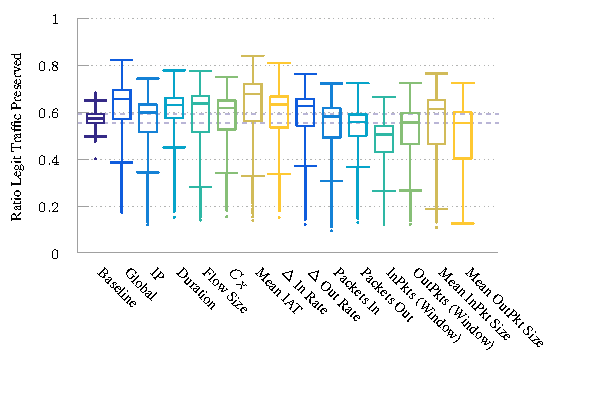
\includegraphics[width=\linewidth]{plots/marl/ftprep-cap-box}
	\caption[Learned performance of \emph{Instant} agents when benign traffic is UDP-like, using only a single feature as a basis for decisions.]{
		Learned performance of \emph{Instant} agents when benign traffic is \gls{acr:udp}-like, using only a single feature as a basis for decisions.
		Mean \gls{acr:iat}, inbound packet sizes, and global state offer the best predictive performance, while most features offer marginal advantage over the unprotected baseline.
		\label{fig:udp-feature-plots}
	}
\end{figure}

\begin{figure}
	\centering
	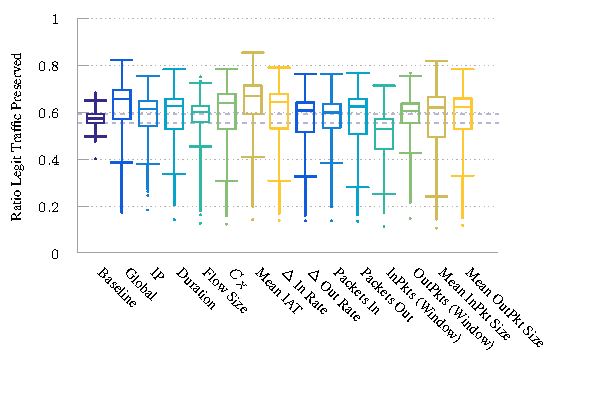
\includegraphics[width=\linewidth]{plots/marl/ftprep-laf-cap-box}
	\caption[Learned performance of \emph{Instant} agents when benign traffic is UDP-like, jointly tiling each feature with the last action taken.]{
		Learned performance of \emph{Instant} agents when benign traffic is \gls{acr:udp}-like, combining each feature with the last action taken as a basis for decisions.
		Compared to \cref{fig:udp-feature-plots}, this combination causes a marked improvement in the packet count and per-window statistics, and leads to a tighter performance bound for Flow Size.
		\label{fig:udp-laf-feature-plots}
	}
\end{figure}

\begin{figure}
	\centering
	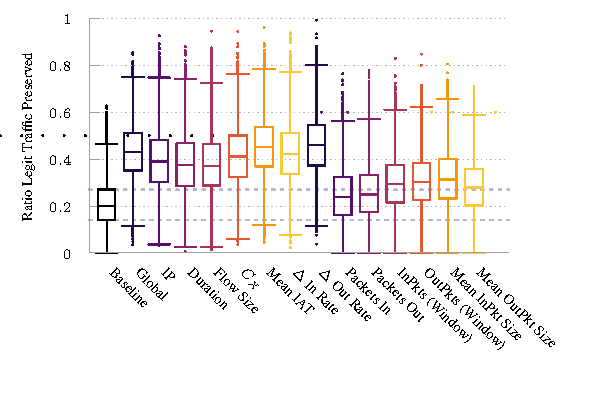
\includegraphics[width=\linewidth]{plots/marl/ftprep-tcp-cap-box}
	\caption[Learned performance of \emph{Instant} agents when benign traffic is TCP-like, using only a single feature as a basis for decisions.]{
		Learned performance of \emph{Instant} agents when benign traffic is \gls{acr:tcp}-like, using only a single feature as a basis for decisions.
		All of the chosen features can offer a marked improvement over no protection at all.
		Global state and Mean \gls{acr:iat} still offer the greatest improvement above baseline, but packet-level statistics are considerably less effective for this class of traffic.
		\label{fig:tcp-cap-feature-plots}
	}
\end{figure}

\begin{figure}
	\centering
%	\vspace{-0.25cm}
	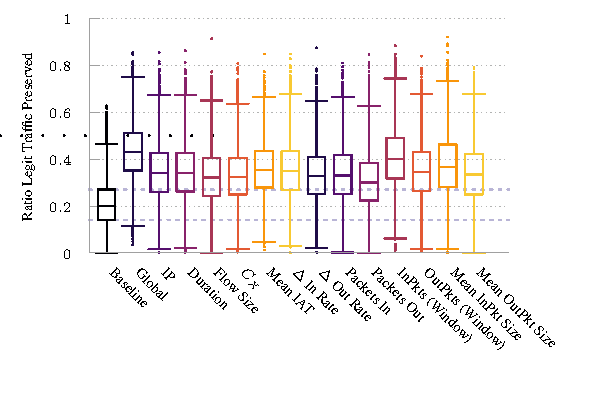
\includegraphics[width=\linewidth]{plots/marl/ftprep-tcp-laf-cap-box}
	\caption[Learned performance of \emph{Instant} agents when benign traffic is TCP-like, jointly tiling each feature with the last action taken.]{
		Learned performance of \emph{Instant} agents when benign traffic is \gls{acr:tcp}-like, combining each feature with the last action taken as a basis for decisions.
		This combination causes a significant improvement in the effectiveness of packet-level and per-window statistics.
		\label{fig:tcp-laf-feature-plots}
	}
\end{figure}

The main element required by a per-source model is a feature set with high predictive power, so that behavioural differences are apparent to an agent.
Elaborating on the statistics discussed in \cref{sec:ddos-motivation} which others have shown to be effective, we believe the following features to be useful (and humanly justifiable), and investigate their use alongside different traffic types.
%?? We use these features, and why...

\paragraph{Global state}
This is the vector of load measurements along a flow's path introduced in \cref{sec:feature-space}.
These values indicate the overall health of the network, and crucially are all measurements which an agent has some degree of direct control over---though the inputs of all agents on all flows are aggregated for later load measurements.

\paragraph{Source IP address}
While trivial to spoof (and thus of limited use for many classes of attack), reflectors are themselves legitimate services being abused by spoofing attackers.
As a result, they communicate with attack victims using their own \gls{acr:ip} address.
In real-world scenarios the addresses of reflector nodes might exhibit similarity due to network uncleanliness~\parencite{DBLP:conf/imc/CollinsSFJWSK07}, e.g., unhardened services exposed by a single organisation.

\paragraph{Last action taken}
This encodes an agent's current belief in the maliciousness of a flow.
This feature also potentially allows forgiveness, serving as a reference point for determining whether a source mistakenly marked as malicious exhibits different falloff behaviour after punishment.
It's important to note that this feature only makes sense once combined with another flow feature, and never appears individually tile-coded.

\paragraph{Flow duration and size}
Features which describe the length of time a connection has been active, and the amount of data transferred within that time.
An extraordinarily long flow, having sent a lot of data, could be more likely to be an amplifier: though most (\qty{62}{\percent}) waves of amplifier traffic last shorter than \qty{15}{\minute}~\parencite{DBLP:conf/raid/KramerKMNKYR15}, this is considerably longer than the typical length of an \gls{acr:http} request/response.

\paragraph{Correspondence ratio}
The ratio between upstream and downstream traffic associated with a source \gls{acr:ip} address.
I define this here as:
$$C_X = \min(\uload{\cdot}, \dload{\cdot})/\max(\uload{\cdot}, \dload{\cdot}),$$
where a value close to 0 indicates strong asymmetry.

\paragraph{$\symbfit{\Delta}$ Send/receive rate}
The change in traffic rates caused by the last action.
Behavioural changes induced by bandwidth expansion or reduction are expected to be most visible here.

\paragraph{Mean inter-arrival time}
A measure of how often packets arrive at the agent's parent switch; low \glspl{acr:iat} indicate a high number of packets per second, and can be a possible marker of malicious behaviour.
I only make use of the mean \gls{acr:iat} of \emph{inbound} traffic.

\paragraph{(Per-window) packet count}
The amount of packets sent to/from a source over a flow's lifetime (or the current window of measurement), similar in use to flow size and mean \gls{acr:iat}.

\paragraph{Mean packet size per window}
Legitimate flows, both congestion-aware and -unaware, often transmit packets with a distribution of sizes.
Attack traffic is not likely to be so diverse: we might expect solely max-size packets in the case of amplification attacks, or minimum-size packets in other flooding attacks.

The exclusion of features such as source/destination ports or protocol numbers is a deliberate choice.
If QUIC or a similar protocol were to become ubiquitous, then these fields would have little to no correlation with the class of traffic a flow might contain.
My aim was to design around this constraint as a form of future-proofing.

\begin{table}
	\centering
	\caption{Tile coding windows for each feature.\label{tab:codings}}
	
%	\resizebox{0.45\linewidth}{!}{
	\begin{tabular}{@{}ll@{}}
		\toprule
		New Feature (unit) & Range \\
		\midrule
		Load (\unit{\mega\bit\per\second}) & $[0, U_s]$ \\
		IP & $[0, 2^{32}-1]$ \\
		Last Action (\unit{\percent}) & $[0, 1]$ \\
		Duration (\unit{\milli\second}) & $[0, \num{2000}]$ \\
		Size (\unit{\mebi\byte}) & $[0,10]$ \\
		Correspondence Ratio & $[0,1]$ \\
		Mean IAT (\unit{\milli\second}) & $[0, \num{10000}]$ \\
		$\Delta$In/Out Rate (\unit{\mega\bit\per\second}) & $[-50, 50]$ \\
		Packets In/Out & $[0, 7000]$ \\
		Packets In/Out Window & $[0, 2000]$ \\
		Mean In/Out Packet Size (\unit{\byte}) & $[0, 1560]$ \\
		\bottomrule
	\end{tabular}
%	}
\end{table}

All of the above features, save for global state, are 1-dimensional.
For simplicity, here `\gls{acr:udp}' refers to congestion-unaware traffic, while `\gls{acr:tcp}' refers to congestion-aware flows.
\Cref{fig:udp-feature-plots} shows the effectiveness of each feature for \gls{acr:udp} (resp.\ \cref{fig:tcp-cap-feature-plots} for \gls{acr:tcp}), on a single-destination topology (\cref{sec:single-dest}) with $n=2$ hosts per egress point averaged over \num{10} runs.
\Cref{fig:tcp-laf-feature-plots} demonstrates how feature accuracy varies when tiled alongside \emph{last action}, with similar trends observed when applied to \gls{acr:udp} traffic (\cref{fig:udp-laf-feature-plots}).
%?? Core findings---different protocols need different features, so everything we proposed above has a use!
The plots show that different protocols and traffic classes are best defended by different features---as such, every feature presented has value in a complete model.
All features converge to their highest-observed performance within around \num{4000} timesteps.
In general, some of the most effective features are the global state, mean \gls{acr:iat}, mean inbound packet size and $\Delta$ rates.
%?? How do they do when combined after individual training? Pretty well, especially for TCP.
%Additional testing shows that the learned per-feature policies may be easily combined (by summing action values), and that this technique is particularly effective for TCP; these results are omitted to preserve space.
%In no cases, however, do we manage to completely block attack traffic---at convergence, we observe that system load remains consistently at $U_s$.